\documentclass[12pt,letterpaper]{article}
\usepackage{graphicx,textcomp}
\usepackage{natbib}
\usepackage{setspace}
\usepackage{fullpage}
\usepackage{color}
\usepackage[reqno]{amsmath}
\usepackage{amsthm}
\usepackage{fancyvrb}
\usepackage{amssymb,enumerate}
\usepackage[all]{xy}
\usepackage{endnotes}
\usepackage{lscape}
\newtheorem{com}{Comment}
\usepackage{float}
\usepackage{hyperref}
\newtheorem{lem} {Lemma}
\newtheorem{prop}{Proposition}
\newtheorem{thm}{Theorem}
\newtheorem{defn}{Definition}
\newtheorem{cor}{Corollary}
\newtheorem{obs}{Observation}
\usepackage[compact]{titlesec}
\usepackage{dcolumn}
\usepackage{tikz}
\usetikzlibrary{arrows}
\usepackage{multirow}
\usepackage{xcolor}
\newcolumntype{.}{D{.}{.}{-1}}
\newcolumntype{d}[1]{D{.}{.}{#1}}
\definecolor{light-gray}{gray}{0.65}
\usepackage{url}
\usepackage{listings}
\usepackage{color}

\definecolor{codegreen}{rgb}{0,0.6,0}
\definecolor{codegray}{rgb}{0.5,0.5,0.5}
\definecolor{codepurple}{rgb}{0.58,0,0.82}
\definecolor{backcolour}{rgb}{0.95,0.95,0.92}

\lstdefinestyle{mystyle}{
	backgroundcolor=\color{backcolour},   
	commentstyle=\color{codegreen},
	keywordstyle=\color{magenta},
	numberstyle=\tiny\color{codegray},
	stringstyle=\color{codepurple},
	basicstyle=\footnotesize,
	breakatwhitespace=false,         
	breaklines=true,                 
	captionpos=b,                    
	keepspaces=true,                 
	numbers=left,                    
	numbersep=5pt,                  
	showspaces=false,                
	showstringspaces=false,
	showtabs=false,                  
	tabsize=2
}
\lstset{style=mystyle}
\newcommand{\Sref}[1]{Section~\ref{#1}}
\newtheorem{hyp}{Hypothesis}

\title{Problem Set 1}
\date{Due: October 1, 2023}
\author{Applied Stats/Quant Methods 1}

\begin{document}
	\maketitle
	
	\section*{Instructions}
	\begin{itemize}
	\item Please show your work! You may lose points by simply writing in the answer. If the problem requires you to execute commands in \texttt{R}, please include the code you used to get your answers. Please also include the \texttt{.R} file that contains your code. If you are not sure if work needs to be shown for a particular problem, please ask.
\item Your homework should be submitted electronically on GitHub.
\item This problem set is due before 23:59 on Sunday October 1, 2023. No late assignments will be accepted.
\item Total available points for this homework is 80.
	\end{itemize}
	
	\vspace{1cm}
	\section*{Question 1 (40 points): Education}

A school counselor was curious about the average of IQ of the students in her school and took a random sample of 25 students' IQ scores. The following is the data set:\\
\vspace{.5cm}

\lstinputlisting[language=R, firstline=37, lastline=37]{PS01.R}  

\vspace{1cm}

\begin{enumerate}
	\item Find a 90\% confidence interval for the average student IQ in the school.\\
	
	\noindent This question is asking to use statistics from a sample (25 random students) to estimate population parameters (the whole school) - in this case, a confidence interval, which is a range of numbers within which the parameter is believed to fall 90\% of the time with repeated sampling. This requires us to assume a normal sampling distribution.
	
	\noindent First I find the point estimate - or sample mean - which is the sum of all the observation values divided by the total number of observations. I also find the sample's n-size.  
	
	\lstinputlisting[language=R, firstline=44, lastline=46]{PS01.R}
	
	\noindent Now I find the sample standard deviation - which is a measure of the spread/dispersion within the sample. This is calculated by first calculating the variance (the sum of the squared distances of each observation from the sample mean (ensuring observations above and below the mean don't cancel out) divided by the total number of observations less one ie n-1). The SD is the square root of the variance, returning the value from squared to original (and more easily comparable) units. I further divide this by the square root of total observations to find the standard error for the sampling distribution ie an estimator for the deviation of sample means with repeated sampling).
	
	\lstinputlisting[language=R, firstline=50, lastline=52]{PS01.R}
	
	\noindent I now define the corresponding p-value for 90\% confidence. Will the calculated values, I can manually approximate the 90\% confidence intervals by multiplying the corresponding Z-score (aka critical value) to the alpha value for 90\% confidence (ie 0.1 including both tails of the distribution, or 0.05 each tail) with the standard error, and then adding/subtracting this figure from the sample mean. In other words, I am adding/subtracting the 'margin for error' to calculate the confidence intervals.
	
	\lstinputlisting[language=R, firstline=56, lastline=59]{PS01.R}
	
	\noindent Alternatively, I can use the qnorm() function to calculate the lower and upper values. This can be more precise if some figures such as z-score or standard deviation/error have been rounded.
	
	\lstinputlisting[language=R, firstline=63, lastline=64]{PS01.R}
	
	\noindent These bounds indicate that, with 90\% confidence with repeated sampling, the population mean (ie the school average IQ) is within the values 94.13 and 102.75 (rounded to two decimal places). 
	
	\item Next, the school counselor was curious  whether  the average student IQ in her school is higher than the average IQ score (100) among all the schools in the country.\\ 
	
	\noindent Using the same sample, conduct the appropriate hypothesis test with $\alpha=0.05$.
	\vspace{.5cm}
	
	\noindent This question requires a significance test for a mean using the t.test() function.
	\vspace{.5cm}
	
	\indent H0: \textit{The average IQ score among all schools (mean\_all) is NOT less than or equal to the average IQ score of our sample (mean\_y).}
	
	HA: \textit{The average IQ score among all schools (mean\_all) IS less than or equal to the sample (mean\_y).}
	\vspace{.5cm}
	
	\lstinputlisting[language=R, firstline=79, lastline=80]{PS01.R}
		
	\begin{verbatim}
		One Sample T-Test
		data: y
		t     = -0.59574     df=24     p-value=0.7215
		
		alternative hypothesis:     true mean is greater than 100
		
		95 percent confidence interval:
		93.95993     Inf
		
		sample estimates:
		mean of x = 98.44
	\end{verbatim}
	
	\noindent The result indicates that p is greater than 0.05, failing to reject the null hypothesis. In full, this means I cannot reject the null hypothesis that the counsellor's school's average IQ score is higher than the average IQ score for all schools.
	
\end{enumerate}

\newpage

	\section*{Question 2 (40 points): Political Economy}

\noindent Researchers are curious about what affects the amount of money communities spend on addressing homelessness. The following variables constitute our data set about social welfare expenditures in the USA. \\
\vspace{.5cm}

\begin{tabular}{r|l}
	\texttt{State} &\emph{50 states in US} \\
	\texttt{Y} & \emph{per capita expenditure on shelters/housing assistance in state}\\
	\texttt{X1} &\emph{per capita personal income in state} \\
	\texttt{X2} &  \emph{Number of residents per 100,000 that are "financially insecure" in state}\\
	\texttt{X3} &  \emph{Number of people per thousand residing in urban areas in state} \\
	\texttt{Region} &  \emph{1=Northeast, 2= North Central, 3= South, 4=West} \\
\end{tabular}

\vspace{.5cm}
\noindent Explore the \texttt{expenditure} data set and import data into \texttt{R}.
\vspace{.5cm}

\lstinputlisting[language=R, firstline=104, lastline=108]{PS01.R}

\begin{itemize}
\item
Please plot the relationships among \emph{Y}, \emph{X1}, \emph{X2}, and \emph{X3}? What are the correlations among them (you just need to describe the graph and the relationships among them)?

\noindent I plot the variables accordingly. Most plots appear to indicate some positive correlation between the two variables. I highlight the correlations between Y and X1, as well as X1 and X2 as being relatively clear. Meanwhile, the (positive) relationship between Y and X3 appears relatively weak or non-existent. I use the png() function to print the plots.

\lstinputlisting[language=R, firstline=117, lastline=120]{PS01.R}
 
 \begin{figure}[H]
 	\centering
 	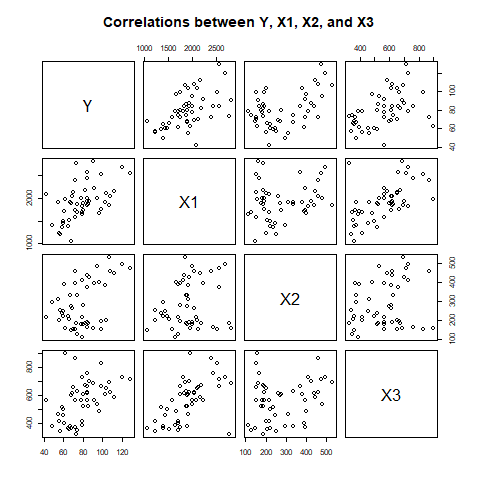
\includegraphics[width=0.5\textwidth]{scatter_y_x1_x2_x3.png}
 	\caption{Relationships across variables: Expenditure on shelters/housing, Personal Income, Number of 'financially insecure' residents, and Number of urban residents}
 \end{figure}

\vspace{.5cm}

\item Please plot the relationship between \emph{Y} and \emph{Region}? On average, which region has the highest per capita expenditure on housing assistance?
\vspace{.5cm}

\noindent First I need to coerce the variable "Region" from integer type to factor type, and then rename the levels to the region names for clarity.

\lstinputlisting[language=R, firstline=127, lastline=128]{PS01.R}

\noindent Now I create a box plot showing expenditure on shelters/housing assistance across region. I then export it as a png.

\lstinputlisting[language=R, firstline=132, lastline=137]{PS01.R}

\noindent The thick black horizontal bars indicate the mean average for each region, indicating the West region has the highest average per capita spending on shelters/housing assistance.

\begin{figure}[H]
	\centering
	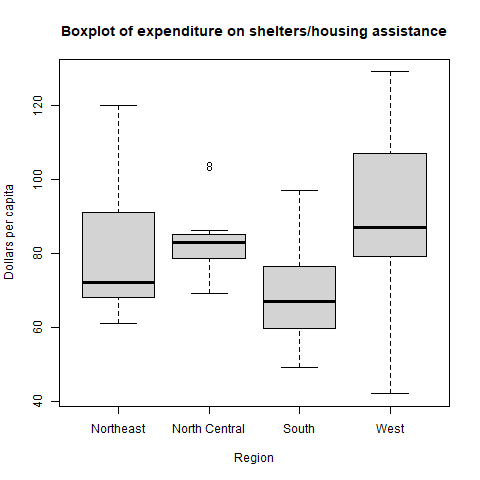
\includegraphics[width=0.5\textwidth]{boxplot_Expenditure_by_Region.png}
	\caption{The Expenditure on shelters/housing assistance by states, across Regions}
\end{figure}

\item
Please plot the relationship between \emph{Y} and \emph{X1}? Describe this graph and the relationship. Reproduce the above graph including one more variable \emph{Region} and display different regions with different types of symbols and colors.

\noindent I produce the first graph, adding a title and axis labels for clarity. The scatter plot indicates a positive relationship between state expenditure on shelters/housing assistance, and personal incomes. I print this first graph as a png.

\noindent Using the function cor(), I find a 0.53 correlation coefficient, indicating a positive correlation and supporting with my visual assessment.

\lstinputlisting[language=R, firstline=148, lastline=154]{PS01.R}

\begin{figure}[H]
	\centering
	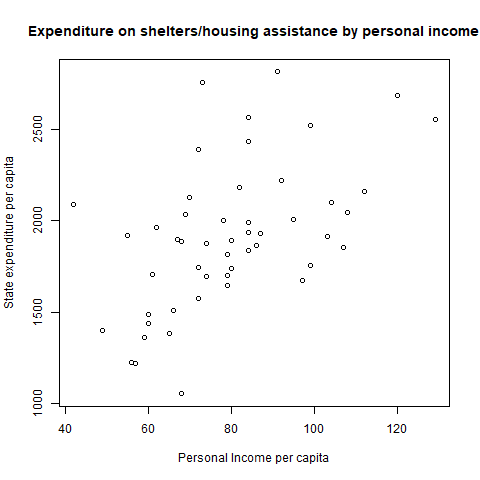
\includegraphics[width=0.5\textwidth]{expenditure_by_personal_income.png}
	\caption{Scatter Plot of Expenditure by Personal Income}
\end{figure}

\noindent Now I reproduce the plot including a legend, with Region indicated by unique symbols and colours.

\lstinputlisting[language=R, firstline=160, lastline=172]{PS01.R}

\begin{figure}[H]
	\centering
	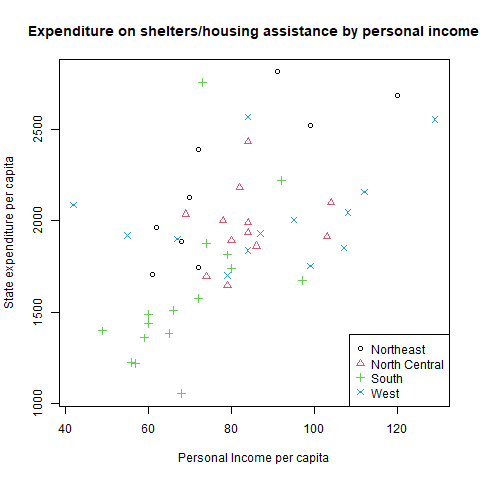
\includegraphics[width=0.5\textwidth]{expenditure_by_personal_income_with_legend.png}
	\caption{Scatter Plot of Expenditure by Personal Income with Legend by Region}
\end{figure}

\noindent Visual indications suggests North Central-states cluster (aka are more similar) with higher state spending AND personal incomes compared to South-states. Meanwhile, West states may have variation in state expenditure compared to personal incomes. No clear associations are indicated for Northeast-states.

\end{itemize}


\end{document}
